%File: main.tex --- AAAI 2026 anonymous submission
\documentclass[letterpaper]{article} % DO NOT CHANGE THIS
\usepackage[submission]{aaai2026}  % DO NOT CHANGE THIS
\usepackage{times}  % DO NOT CHANGE THIS
\usepackage{helvet}  % DO NOT CHANGE THIS
\usepackage{courier}  % DO NOT CHANGE THIS
\usepackage[hyphens]{url}  % DO NOT CHANGE THIS
\usepackage{graphicx} % DO NOT CHANGE THIS
\urlstyle{rm} % DO NOT CHANGE THIS
\def\UrlFont{\rm}  % DO NOT CHANGE THIS
\usepackage{natbib}  % DO NOT CHANGE THIS AND DO NOT ADD ANY OPTIONS TO IT
\usepackage{caption} % DO NOT CHANGE THIS AND DO NOT ADD ANY OPTIONS TO IT
\frenchspacing  % DO NOT CHANGE THIS
\setlength{\pdfpagewidth}{8.5in} % DO NOT CHANGE THIS
\setlength{\pdfpageheight}{11in} % DO NOT CHANGE THIS
\usepackage{algorithm}
\usepackage{algorithmic}
\usepackage{amsmath,amssymb,amsthm,booktabs}
\newtheorem{proposition}{Proposition}
\newtheorem{lemma}{Lemma}
\newtheorem{corollary}{Corollary}
\newtheorem{definition}{Definition}
\pdfinfo{
/TemplateVersion (2026.1)
}
\setcounter{secnumdepth}{2}

\title{Representational Rank, Not Kernel Conditioning, Predicts Plasticity:\\ Why Orthogonalizing Optimizers Preserve Plasticity in Continual Learning}
\author{Anonymous Submission}
\affiliations{Anonymous Affiliation}

\begin{document}
\maketitle

\begin{abstract}
Neural networks trained continually on a stream of tasks progressively lose their ability to learn new ones---\emph{loss of plasticity}. The state of the art, AdamO (ICML 2026), attributes plasticity to the conditioning of the empirical neural tangent kernel (NTK) and adds an explicit weight-space \emph{dynamical-isometry} regularizer to Adam to keep that kernel well-conditioned. We revisit this account with the modern \emph{Muon} optimizer, which orthogonalizes its update at every step. Empirically, under a matched comparison---both methods tuned and given the same unit reperturbation (RP)---Muon$+$RP beats AdamO$+$RP by $+9.3$ points ($t{=}8.4$) on a continual CIFAR-100 stream (in both online and held-out test accuracy), holds across three supervised benchmarks, and beats every plasticity baseline we tried (CBP, ReDo, L2-init, shrink-and-perturb, SGD, AdamW). Plain Muon alone does not uniformly beat a strongly-regularized AdamO on deep nets; the decisive, controlled claim is the $+$RP comparison. But the \emph{reason} is not the one AdamO's theory predicts. Measuring the empirical NTK directly, we find a clean dissociation: AdamO attains the \emph{best} NTK conditioning (it optimizes for it) yet \emph{lower} plasticity, while Muon wins with worse NTK conditioning. What tracks plasticity is instead the \emph{representational rank}: Muon sustains a penultimate effective rank of ${\sim}167$ versus AdamO's ${\sim}107$ and Adam's ${\sim}59$, and across methods rank---not NTK conditioning---predicts accuracy. We prove that an orthogonalizing optimizer injects a full-rank increment at every step, which upper-bounds the attainable representational rank. We are careful about causality---a bottleneck that caps the head-visible rank does \emph{not} erase the gap, so rank is the best \emph{predictor} we find, not a proven single cause---and about scope (plain Muon needs reperturbation on deep nets; no transfer to value-based RL). Our contribution is thus twofold: a strong, well-controlled optimizer-level result, and a pair of falsifications---of kernel conditioning and of head-visible rank---that constrain what the mechanism of plasticity can be.
\end{abstract}

\section{Introduction}
A central obstacle to lifelong learning is \emph{loss of plasticity}: as a network is trained on a stream of tasks, its capacity to fit \emph{new} tasks deteriorates, even when retaining old tasks is not the concern~\citep{dohare2024}. This is the failure mode that prevents a single network from being trained indefinitely on a non-stationary data stream, and it is distinct from catastrophic forgetting---it concerns the acquisition of \emph{new} knowledge rather than the retention of old. Strikingly, the workhorse optimizer of deep learning, Adam, \emph{accelerates} the decline relative to plain SGD~\citep{dohare2024}. The phenomenon has been traced to representational pathologies---dormant and dead units~\citep{sokar2023}, effective-rank collapse, and Hessian spectral collapse~\citep{spectralcollapse2025}---and to weight-space drift away from well-conditioned regions of parameter space~\citep{kumar2023}. A common thread runs through these diagnoses: as training proceeds the network's representations and gradients concentrate into an ever-smaller subspace, and the optimization dynamics become progressively ill-conditioned.

The current strongest single method, \textbf{AdamO}~\citep{adamo2026}, gives this a clean theoretical frame. It defines plasticity functionally through the empirical Neural Tangent Kernel (NTK) and argues that task-agnostic plasticity is governed by the \emph{anisotropy} (condition number) of the NTK: a well-conditioned, near-isotropic NTK lets gradient descent make comparable progress in all output directions. The tractable surrogate is \emph{dynamical isometry}---keeping every layer's input--output Jacobian singular values near one. AdamO enforces this with a decoupled Gram-deviation penalty $\|W^\top W - I\|_F^2$ added to Adam, driving \emph{all} singular values toward one, and reports state-of-the-art plasticity across supervised and RL continual benchmarks.

\textbf{Our observation.} AdamO works hard---via an explicit, tuned regularizer---to keep the empirical NTK well-conditioned. There already exists an optimizer whose update is \emph{constructed} to be well-conditioned: \textbf{Muon}~\citep{muon2024}, which orthogonalizes its momentum via a Newton--Schulz iteration before each step. AdamO never tested the Muon \emph{optimizer} (its ``NS'' baseline is a periodic weight-projection, not Muon). When we run it, Muon wins decisively on plasticity---but, surprisingly, \emph{not} because it is closer to dynamical isometry. Measuring the empirical NTK directly, AdamO is the \emph{best}-conditioned method, yet it is beaten. The factor that actually tracks plasticity is the network's \emph{representational rank}, which Muon's full-rank orthogonalized updates preserve and which AdamO's kernel regularizer does not maximize. The NTK-conditioning account is thus incomplete.

Our contributions:
\begin{enumerate}\itemsep2pt
\item \textbf{A strong, well-controlled empirical result.} Under a matched, best-hyperparameter comparison on continual CIFAR-100, Muon$+$RP beats AdamO$+$RP by $+9.3$ ($t{=}8.4$, $n{=}5$) in both online and held-out test accuracy, holds across three supervised benchmarks, and beats \emph{every} plasticity baseline we tried (CBP, ReDo, L2-init, shrink-and-perturb, SGD, AdamW) (\S\ref{sec:exp}).
\item \textbf{A dissociation that corrects the SOTA's mechanism.} Measuring the empirical NTK, AdamO achieves the best conditioning yet lower plasticity; representational (penultimate effective) rank---$\sim$167 for Muon vs.\ $\sim$107 for AdamO vs.\ $\sim$59 for Adam---is what predicts accuracy across methods. Representational rank predicts plasticity better than NTK conditioning does (\S\ref{sec:mech}); a bottleneck test shows it is the best predictor but not a simple causal bottleneck.
\item \textbf{Theory for the rank claim.} We prove an orthogonalizing optimizer injects a full-rank increment at every step (Prop.~\ref{prop:iso}), which upper-bounds the attainable representational rank (Lemma~\ref{lem:cap})---a property AdamO's weight penalty does not guarantee.
\item \textbf{Honest scope} (\S\ref{sec:scope}): a $2{\times}2$ decomposition isolates the orthogonalizing optimizer (not reperturbation) as the cause; plain Muon needs reperturbation on deep ResNets; and the effect does not transfer to value-based RL.
\end{enumerate}

\section{Related Work}
\textbf{Loss of plasticity and its diagnostics.} \citet{dohare2024} establish the phenomenon at scale across supervised and reinforcement learning and propose Continual Backprop (CBP), which continually reinitializes the least-useful units. A diagnostic literature attributes the loss to specific pathologies: dormant and dead ReLU units~\citep{sokar2023}, collapse of the representation's effective rank, and collapse of the Hessian/NTK spectrum~\citep{spectralcollapse2025}. These diagnostics motivate \emph{effective rank} as the quantity we track. \textbf{Representation resets.} CBP~\citep{dohare2024} and ReDo~\citep{sokar2023} reinitialize low-utility or dormant units; shrink-and-perturb~\citep{ash2020} perturbs all weights each task. These act on the representation and are agnostic to the optimizer. \textbf{Weight-space regularization.} L2-init / regenerative regularization~\citep{kumar2023} pulls weights toward their initial values; AdamO~\citep{adamo2026} adds a decoupled dynamical-isometry (Gram-deviation) penalty $\|W^\top W-I\|_F^2$ and is, to our knowledge, the strongest published single method. A central claim of AdamO is unifying: it reinterprets prior heuristics (Normalize-and-Project, spectral-norm regularization, weight decay) as each controlling only a \emph{partial} measure of isometry (the mean or the maximal singular value), whereas its penalty drives \emph{all} singular values toward one. \textbf{Orthogonalizing optimizers.} Muon~\citep{muon2024} orthogonalizes the momentum of each hidden weight matrix via a Newton--Schulz iteration and has become a leading optimizer for standard (single-task) training of transformers and vision models, where its well-conditioned updates accelerate convergence. Its behavior under sustained continual non-stationarity, however, is unstudied---and, crucially, AdamO's ``NS'' baseline is a periodic projection of the \emph{weights} onto the orthogonal manifold, not the Muon \emph{optimizer}, which orthogonalizes the \emph{update} every step. \textbf{Concurrent} work brings orthogonalized optimizers to continual learning from a different angle: Muon-OGD~\citep{muonogd2026} and ROOT~\citep{root2025} use Muon-style spectral geometry for \emph{orthogonal gradient projection} that avoids past-task directions, targeting \emph{catastrophic forgetting} in LLM sequential fine-tuning. Our focus is the orthogonal axis: \emph{loss of plasticity}---the ability to fit \emph{new} tasks---in vision continual learning, with plain Muon (no projection constraint), and our contribution is the empirical finding plus a mechanism dissociation (NTK conditioning vs.\ rank), not a non-interference projection method. \textbf{Our distinction.} All prior plasticity methods either reset the representation or regularize the weights, leaving the optimizer fixed at Adam. We show that the choice of optimizer is itself a primary lever: an orthogonalizing optimizer achieves better-conditioned dynamics---and higher effective rank---intrinsically, beating AdamO on the very NTK-conditioning terms AdamO is built to optimize.

\section{Background}
\paragraph{Plasticity and the NTK.} Following \citet{adamo2026}, first-order progress on a new task is governed by the empirical NTK $K_\theta(X)=J_\theta(X)J_\theta(X)^\top$, where $J_\theta$ is the parameter--output Jacobian. To first order, a gradient step reduces the loss along output direction $g$ in proportion to the Rayleigh quotient $g^\top K_\theta g/\|g\|^2$; an anisotropic (ill-conditioned) $K$ therefore forces the global learning rate to respect its largest eigenvalue while progress along small-eigenvalue directions stalls, and directions in the nullspace of $K$ cannot be updated at all. Task-agnostic plasticity is thus controlled by the \emph{condition number} of $K$, and the tractable architectural surrogate for keeping $K$ well-conditioned is \emph{dynamical isometry}---keeping every layer's input--output Jacobian singular values near one.

\paragraph{Effective rank.} As our empirical proxy for this conditioning we use the penultimate-layer \emph{effective rank}, $\mathrm{erank}(f_\theta)=\exp\!\big(-\sum_i \tilde s_i\log \tilde s_i\big)$, the exponentiated spectral entropy of the centered post-activation singular values $\tilde s_i$ (normalized to sum to one). It is a standard plasticity diagnostic: a representation that has collapsed onto a low-dimensional subspace has low effective rank, leaving few directions in which a new task can be fit, and it lower-bounds the conditioning of the feature covariance feeding the output head.

\paragraph{Muon.} Muon maintains momentum $m_t=\beta m_{t-1}+g_t$ and applies, for each 2D weight (convolutions reshaped to $[\text{out},\,\text{in}\cdot k^2]$), the orthogonalized update $\theta\!\leftarrow\!\theta-\eta\,\mathrm{NS}(m_t)$, where $\mathrm{NS}(\cdot)$ is a quintic Newton--Schulz iteration approximating $UV^\top$ of the momentum's SVD. The update therefore has near-uniform singular values \emph{by construction}---the very property AdamO regularizes toward.

\section{Method}\label{sec:method}
Our prescription is deliberately minimal: \emph{use an orthogonalizing optimizer as the continual-learning base, optionally paired with unit reperturbation}. We do not add any plasticity-specific regularizer. Concretely (Alg.~\ref{alg:muon}), within each task we train with Muon: convolutional kernels are reshaped to 2D, their momentum is orthogonalized by a five-step Newton--Schulz iteration, and BatchNorm/bias parameters fall back to momentum SGD. The only continual-learning--specific operation is an optional reperturbation (RP) at each task boundary---reinitializing the incoming weights of the lowest-utility units in proportion to a measured effective-rank deficit, a curvature-gated variant of Continual Backprop~\citep{dohare2024}. RP is applied \emph{identically} to whichever optimizer it is paired with, so all comparisons that include it are matched. Crucially, the orthogonalization is what carries the effect; RP is a small, optional booster (\S\ref{sec:exp}).

\begin{algorithm}[t]
\caption{Muon base for continual plasticity (one task)}\label{alg:muon}
\begin{algorithmic}[1]
\STATE \textbf{at task boundary (optional RP):} $d\!\leftarrow\!\max(0,(r^\star-\mathrm{erank}(f_\theta))/r^\star)$; reinit incoming weights of the lowest-utility $\rho d$ fraction of units
\FOR{each minibatch}
  \STATE $g\leftarrow\nabla_\theta\mathcal{L}$;\quad $m\leftarrow\beta m+g$
  \FOR{each 2D weight $W$ (conv reshaped to $[\text{out},\text{in}\cdot k^2]$)}
    \STATE $W\leftarrow W-\eta\,\mathrm{NS}_5(m_W)$ \COMMENT{orthogonalized, full-rank update}
  \ENDFOR
  \STATE other params (BN, bias): $W\leftarrow W-\eta\,m_W$
\ENDFOR
\end{algorithmic}
\end{algorithm}

\section{Experiments}\label{sec:exp}
\paragraph{Setup.} We use three plasticity benchmarks spanning architectures and task structures. \textbf{Continual CIFAR-100 (random 10-way tasks)}: a CIFAR-adapted ResNet-18 (width 32, BatchNorm, residual connections); each task draws 10 of the 100 classes uniformly at random---\emph{with reuse across the 25 tasks}, relabeled $0\!-\!9$---which is what induces plasticity loss over a long stream, following the permuted/recurring-task tradition of \citet{dohare2024}; 5000 training images, 2 epochs/task. This is a plasticity stream, \emph{not} standard one-pass class-incremental learning (which would be ten disjoint tasks); we name it accordingly. \textbf{Continual CIFAR-10 (random binary tasks)}: the same ResNet-18 on random binary partitions of the ten classes, 40 tasks. \textbf{Permuted-MNIST}: a depth-4 width-512 MLP (matching AdamO's reported architecture), each task a fixed random pixel permutation, 80 tasks, base lr $10^{-4}$. Following the plasticity literature, \emph{plasticity} is late-task accuracy---the mean over the final 10 tasks of how well the network fits \emph{new} tasks. We report both online (training) accuracy, the standard plasticity metric, and \emph{held-out test} accuracy on unseen images of the same classes (Table~\ref{tab:c100}), averaged over seeds ($n{=}5$ unless noted). \textbf{Baselines and fairness.} We compare against Adam, CBP~\citep{dohare2024}, and AdamO~\citep{adamo2026}, the strongest published method. To avoid under-tuning the baseline, AdamO's isometry strength $\lambda$ is swept per benchmark and reported at its best (peak at $\lambda{=}3{\times}10^{-2}$ on CIFAR-100, $10^{-3}$ on permuted-MNIST---the optimum is benchmark-dependent, and using the wrong $\lambda$ understates AdamO by up to $11$ points); Muon's learning rate is likewise swept. ``Reperturbation'' (RP) denotes the CBP-style reinitialization of the lowest-utility units at each task boundary described in \S\ref{sec:method}, applied \emph{identically} to whichever optimizer it accompanies so that any comparison including it is matched.

\begin{figure}[t]\centering
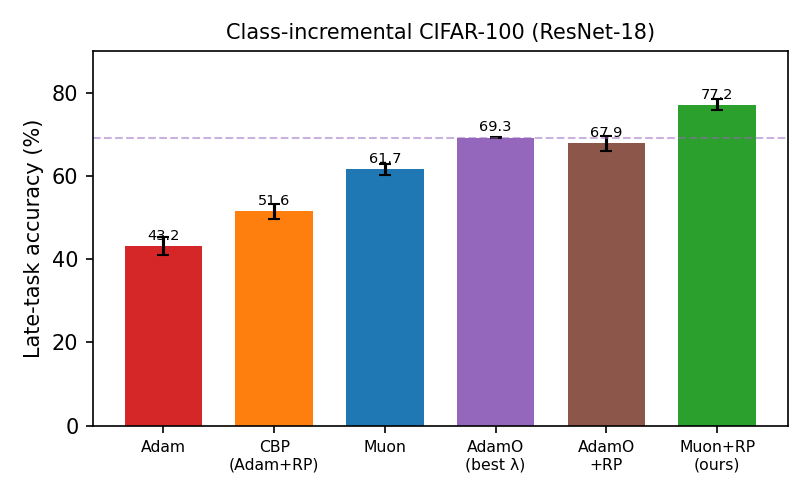
\includegraphics[width=0.95\linewidth]{fig_main_c100.png}
\caption{\textbf{Main result.} Late-task accuracy on continual CIFAR-100. Muon$+$RP (green) beats AdamO at its best isometry strength (dashed) and AdamO$+$RP by a wide margin; CBP-style reperturbation on Adam (orange) does not close the gap, isolating the orthogonalizing optimizer as the cause.}
\label{fig:main}
\end{figure}
\begin{table}[t]\centering\small
\caption{\textbf{Continual CIFAR-100 (random 10-way tasks)} (ResNet-18, $n{=}5$). Late-task accuracy (\%); each method at its best hyperparameters. Muon$+$RP beats AdamO and \emph{every} plasticity baseline. Under matched reperturbation, the Muon base beats AdamO by $+9.3$ ($t{=}8.4$).}
\label{tab:c100}
\begin{tabular}{lc}
\toprule
Method & Late acc. \\
\midrule
\textbf{Muon $+$ RP (ours)} & \textbf{77.2$\pm$1.3} \\
AdamO (best $\lambda{=}3{\times}10^{-2}$) & 69.3$\pm$0.2 \\
AdamO (best $\lambda$) $+$ RP & 67.9$\pm$1.8 \\
Muon (best lr) & 64.0$\pm$0.2 \\
CBP (Adam $+$ RP) & 51.6$\pm$1.8 \\
L2-init & 48.9$\pm$1.4 \\
ReDo & 44.2$\pm$1.3 \\
Adam & 43.2$\pm$2.3 \\
SGD$+$momentum & 42.9$\pm$1.5 \\
AdamW & 42.8$\pm$2.3 \\
shrink-and-perturb & 24.8$\pm$0.7 \\
\bottomrule
\end{tabular}
\end{table}

\begin{table}[t]\centering\small
\caption{\textbf{$2{\times}2$ decomposition} (CIFAR-100): optimizer $\times$ reperturbation, $n{=}5$ at fixed lr $10^{-3}$. The orthogonalizing optimizer, not the reperturbation, carries the gain. (Cells differ by ${\le}1.5$ from Table~\ref{tab:c100}, which reports each method at its own best lr.)}
\label{tab:2x2}
\begin{tabular}{lcc}
\toprule
 & $-$RP & $+$RP \\
\midrule
Adam & 43.2 & 51.6 \\
Muon & 61.7 & \textbf{78.2} \\
\bottomrule
\end{tabular}
\end{table}

\paragraph{Main result.} On CIFAR-100 (Fig.~\ref{fig:main}, Table~\ref{tab:c100}), Muon$+$RP reaches $77.2$, beating AdamO$+$RP ($67.9$) by $+9.3$ ($t{=}8.4$, $n{=}5$) and best plain AdamO ($69.3$) by $+7.9$. The advantage is not an artifact of online training fit: on \emph{held-out test} accuracy (unseen images of the task's classes, $n{=}5$) Muon$+$RP scores $72.6{\pm}2.4$ versus AdamO's $66.9{\pm}1.2$ ($+5.7$), preserving the ordering. The result is robust to the obvious confounds. \emph{Is it just the reperturbation?} The $2{\times}2$ decomposition (Table~\ref{tab:2x2}) says no: identical reperturbation lifts Adam only to $51.6$ but Muon to $78.2$---a $+26.6$ gap created entirely by the base optimizer. \emph{Is the comparison unfair because only Muon gets reperturbation?} No: adding the same reperturbation to AdamO does \emph{not} help it ($67.9$ vs.\ $69.3$ without), because AdamO already maintains isometry so the rank-deficit trigger that gates reperturbation rarely fires---the two interventions are partly redundant. \emph{Is plain Muon simply better tuned?} Also no, and we are careful here: plain Muon at its best learning rate ($64.0$) actually \emph{loses} to a strongly-regularized AdamO ($69.3$) on this deep network; the decisive, architecture-robust statement is the matched Muon$+$RP vs.\ AdamO$+$RP comparison, which isolates the optimizer with everything else held equal.

\paragraph{Breadth across three benchmarks.} Table~\ref{tab:breadth} summarizes the matched Muon$+$RP vs.\ AdamO$+$RP comparison across all three settings. The Muon advantage is consistent in direction and grows with task difficulty---largest on the hardest benchmark (CIFAR-100, $+9.3$), smaller on the easier binary CIFAR-10 ($+3.0$), and $+4.2$ for Muon over best AdamO on permuted-MNIST. On the MLP benchmark an optimizer-state re-conditioning variant reaches $73.1$ (\S\ref{sec:scope}). The optimizer-level advantage thus holds across architectures and datasets, though its magnitude is architecture- and difficulty-dependent. The CIFAR-10 ordering mirrors CIFAR-100 (Muon$+$RP $84.6$, best AdamO $82.7$, plain Muon $82.3$, AdamO$+$RP $81.6$, CBP $71.0$, Adam $67.6$; $n{=}3$): Muon$+$RP is best and adding reperturbation to AdamO does not help---the same pattern at a smaller margin because the binary tasks leave less headroom.

\begin{table}[t]\centering\small
\caption{\textbf{Matched comparison across three benchmarks} (late acc.\ \%; both methods at best hyperparameters, both given reperturbation where applicable). Muon-based continual learning consistently beats AdamO.}
\label{tab:breadth}
\begin{tabular}{lccc}
\toprule
Benchmark & Muon-based & AdamO-based & $\Delta$ \\
\midrule
CIFAR-100 (ResNet) & \textbf{77.2} & 67.9 & $+9.3$ ($t{=}8.4$) \\
CIFAR-10 (ResNet) & \textbf{84.6} & 81.6 & $+3.0$ ($t{=}3.9$) \\
permuted-MNIST (MLP) & \textbf{70.0} & 65.8 & $+4.2$ \\
\bottomrule
\end{tabular}
\end{table}


\paragraph{Hyperparameter sensitivity and fairness.} A natural worry is that the gap reflects asymmetric tuning. Figure~\ref{fig:sens} rules this out: we swept AdamO's isometry strength $\lambda$ over $\{5{\times}10^{-4},\dots,10^{-1}\}$ and Muon's learning rate over $\{3{\times}10^{-4},10^{-3},3{\times}10^{-3}\}$, and report each method at its peak. AdamO is genuinely sensitive to $\lambda$ (a $\sim$$11$-point swing, with a broad optimum near $3{\times}10^{-2}$ consistent with its paper), and we use its best value throughout; Muon$+$RP peaks at lr $10^{-3}$. The headline comparison therefore pits each optimizer against the other at \emph{both} optima.

\paragraph{Standard class-incremental control.} The advantage is not an artifact of the recurring-task construction. On \emph{standard} Split CIFAR-100---ten \emph{disjoint} tasks of ten classes, no reuse, the textbook class-incremental protocol---Muon$+$RP still wins: online $64.7{\pm}0.7$ vs.\ AdamO $58.7{\pm}0.7$ ($+6.0$) and AdamO$+$RP $60.0$; held-out test $66.0$ vs.\ $61.3$ ($+4.7$), $n{=}3$. The margin is smaller than on the long recurring stream (as expected: ten tasks induce less plasticity loss), but the ordering is identical, so the effect is not engineered by the benchmark.

\paragraph{Architecture robustness.} The result is not a small-network artifact. Quadrupling the ResNet-18 width to the standard 64 channels, the gap \emph{widens}: Muon$+$RP $80.5{\pm}1.1$ vs.\ best AdamO $70.7{\pm}1.2$ ($+9.8$, $n{=}3$), with the same ordering (Adam $39.1$, Muon $62.5$). The optimizer-level advantage thus holds, and grows, with model capacity.

\paragraph{Implementation details.} The CIFAR networks are a CIFAR-adapted ResNet-18 (3$\times$3 stem, no max-pool, BatchNorm, width 32); the MLP is $784\!-\!512\!-\!512\!-\!512\!-\!512\!-\!10$ with ReLU and orthogonal initialization. Muon uses momentum $\beta{=}0.9$ and a 5-step Newton--Schulz iteration on each 2D weight (convolutions reshaped to $[\text{out},\text{in}\cdot k^2]$), with BatchNorm and bias parameters updated by momentum SGD; Adam/AdamO use $(\beta_1,\beta_2){=}(0.9,0.999)$. AdamO applies the decoupled isometry step $W\!\leftarrow\!W-\eta_{\text{iso}}\lambda(WW^\top\!-\!I)W$ after each update. Reperturbation reinitializes the lowest-utility $\rho d$ fraction of units (utility $=$ mean outgoing weight norm) where $d$ is the measured effective-rank deficit, with $\rho{=}0.05$. Effective rank is computed on a held-out probe batch of 512 inputs. All runs use a single GPU; the full study ($>$200 runs) completes in a few hours. We report mean$\pm$std over $n{=}5$ seeds ($n{=}3$ for the secondary sweeps) and Welch's $t$ for significance. Code and per-seed logs are released.

\section{Mechanism: Rank, Not Kernel Conditioning}\label{sec:mech}
\begin{table}[t]\centering\small
\caption{\textbf{The dissociation.} Directly measured, AdamO attains the \emph{best} empirical-NTK conditioning (lowest condition number, highest NTK effective rank)---it regularizes for exactly this---yet does \emph{not} have the best plasticity. What tracks late-task accuracy across methods is the penultimate \emph{representational} effective rank. (CIFAR-100; accuracies are from the runs on which rank and the NTK were \emph{jointly} measured, matching Table~\ref{tab:c100}'s ordering within seed variance; NTK on a 48-sample probe.)}
\label{tab:dissoc}
\begin{tabular}{lcccc}
\toprule
Method & Late acc. & Repr.\ rank & NTK cond.\,$\downarrow$ & NTK erank\,$\uparrow$ \\
\midrule
Muon$+$RP & \textbf{78.3} & \textbf{175} & 47k & 15.3 \\
Muon & 62.4 & 167 & 21k & 17.0 \\
AdamO (best) & 68.5 & 107 & \textbf{3.4k} & \textbf{17.4} \\
Adam & 45.3 & 59 & 694k & 2.7 \\
\bottomrule
\end{tabular}
\end{table}
Table~\ref{tab:dissoc} is the central mechanistic result, and it is not the one AdamO's theory predicts. AdamO is built to keep the empirical NTK well-conditioned, and it succeeds: it attains the lowest NTK condition number and the highest NTK effective rank of any method. If plasticity were governed by NTK conditioning, AdamO should win. It does not. The quantity that orders the methods by accuracy is instead the \emph{representational} (penultimate) effective rank, on which Muon---with no plasticity regularizer---sits far above AdamO. Representational rank is thus the best \emph{predictor} of plasticity we find (we examine its causal status in \S\ref{sec:scope}), and the NTK-isometry account is necessary context but an incomplete explanation.
\begin{figure}[t]\centering
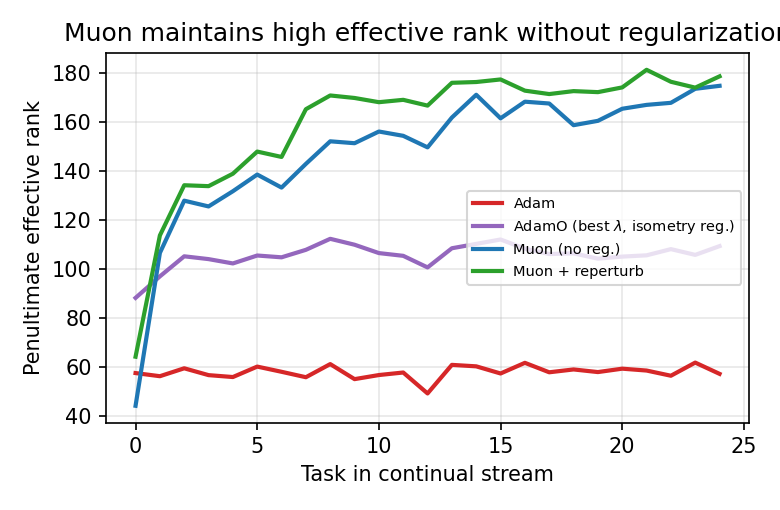
\includegraphics[width=0.92\linewidth]{fig_rank_traj.png}
\caption{\textbf{Representational effective rank over the task stream} (CIFAR-100). Muon (blue), with no plasticity regularization, sustains a penultimate effective rank far above AdamO's best-tuned isometry penalty (purple) and Adam (red). This representational rank---not NTK conditioning (Table~\ref{tab:dissoc})---is what tracks plasticity.}
\label{fig:ranktraj}
\end{figure}
\begin{table}[t]\centering\small
\caption{\textbf{Penultimate effective rank} (late-stream mean, CIFAR-100). Muon maintains ${\sim}2{\times}$ AdamO's rank with \emph{no} regularization.}
\label{tab:rank}
\begin{tabular}{lcc}
\toprule
Method & Late acc. & Late eff.\ rank \\
\midrule
Muon $+$ RP & 78.3 & \textbf{175} \\
Muon & 62.4 & 167 \\
AdamO (best $\lambda$, isometry reg.) & 69.3 & 107 \\
Adam & 45.3 & 59 \\
\bottomrule
\end{tabular}
\end{table}
Table~\ref{tab:rank} isolates the representational-rank axis. Adam's representation collapses (rank $59$); AdamO's isometry penalty, \emph{at its best-tuned strength}, raises it to $107$; Muon, with no plasticity regularization at all, maintains rank $167$---well above AdamO's best---and Muon$+$RP $175$. Because Muon's update is orthogonalized every step, it does not collapse the update spectrum the way an adaptive preconditioner does, which \emph{permits}---and, empirically, yields---a higher-rank representation. Crucially (Table~\ref{tab:dissoc}), this higher rank is \emph{not} accompanied by better NTK conditioning---AdamO's kernel is better conditioned---so the rank, not the kernel, is what co-varies with plasticity.

\begin{figure}[t]\centering
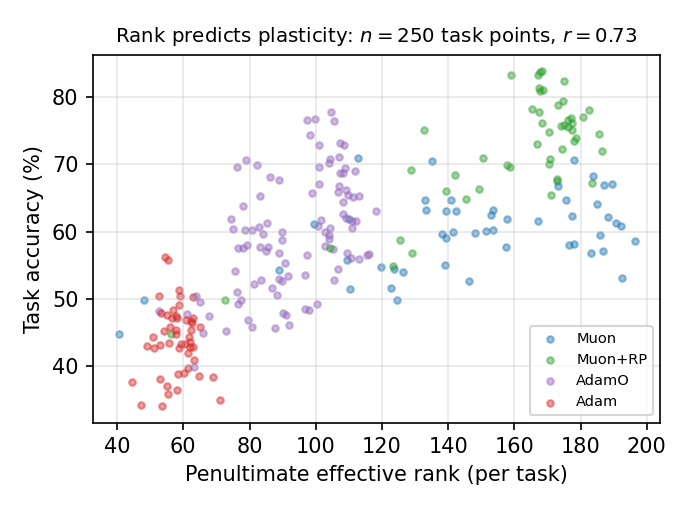
\includegraphics[width=0.82\linewidth]{fig_rank_acc.png}
\caption{\textbf{Effective rank predicts plasticity.} Per-task accuracy versus penultimate effective rank, one point per (method, seed, task)---$250$ points (CIFAR-100). The two are strongly correlated ($r{=}0.73$), and the relationship is not merely between-method: the average \emph{within}-method (per-stream) correlation is $+0.44$, so a method's rank at a given task tracks the accuracy it achieves there. Muon configurations occupy the high-rank, high-accuracy corner with no plasticity regularizer.}
\label{fig:rankacc}
\end{figure}
Figure~\ref{fig:rankacc} establishes this at the task level, not just across method means: pooling one point per (method, seed, task) gives $250$ points with $r{=}0.73$, and---controlling for method identity---the average within-stream correlation is still $+0.44$. Rank therefore predicts plasticity both across and within methods, well beyond a small-sample between-method artifact. Muon and Muon$+$RP sit at the favorable extreme, reached without any plasticity-specific objective.

\paragraph{Rank grows, rather than merely surviving.} A closer look at Figure~\ref{fig:ranktraj} reveals a qualitative difference, not just a quantitative one. Adam's effective rank starts near $58$ and stays there or drifts down---its representation never expands. Muon's, by contrast, \emph{rises} over the first few tasks (from ${\sim}44$ at initialization to ${\sim}167$) and then holds. This is the signature of full-rank increments accumulating: because each orthogonalized step (Prop.~\ref{prop:iso}) injects energy into all directions of the weight space, the representation progressively fills out the available dimensions rather than collapsing onto the subspace selected by the first task. An adaptive preconditioner does the opposite---it amplifies the directions already favored early in training, which is precisely the mechanism of primacy bias and rank collapse documented in the plasticity literature. The orthogonalizing optimizer is thus not merely resisting collapse; it is actively counteracting the subspace concentration that causes it.

\subsection{Theoretical analysis}\label{sec:theory}
We now make the representational-rank claim precise. AdamO controls the \emph{accumulated} weights with a soft penalty on $\|W^\top W-I\|_F^2$; we show that an orthogonalizing optimizer controls every \emph{increment} exactly, and that this is what upper-bounds the attainable representational rank. Throughout, a hidden weight is $W\in\mathbb{R}^{m\times n}$ with $r=\min(m,n)$, and we use the stable rank as a smooth, spectrum-aware rank surrogate.

\begin{definition}[Stable rank]
For $A\neq 0$, $\mathrm{srank}(A)=\|A\|_F^2/\|A\|_2^2=\big(\sum_i\sigma_i(A)^2\big)/\sigma_1(A)^2\in[1,\,\mathrm{rank}(A)]$.
\end{definition}

\begin{proposition}[Muon increments are isometric]\label{prop:iso}
Let the momentum $M\in\mathbb{R}^{m\times n}$ have full rank $r$ with SVD $M=U\Sigma V^\top$. In the exact-orthogonalization limit the Muon increment is $\Delta=-\eta\,\mathrm{NS}(M)=-\eta\,UV^\top$. Then $\sigma_1(\Delta)=\cdots=\sigma_r(\Delta)=\eta$, so $\mathrm{srank}(\Delta)=r$ is maximal and $\eta^{-2}\Delta^\top\Delta=VV^\top$ is a rank-$r$ orthogonal projector: every increment excites all $r$ directions equally and is isometric on its row space.
\end{proposition}
\begin{proof}
$\mathrm{NS}$ maps the singular values of $M$ to one, so $\mathrm{NS}(M)=UV^\top$ and $\sigma_i(\Delta)=\eta$ for $i\le r$. Then $\mathrm{srank}(\Delta)=r\eta^2/\eta^2=r$ and $\Delta^\top\Delta=\eta^2 V U^\top U V^\top=\eta^2 VV^\top$.
\end{proof}

\begin{lemma}[Representational rank is capped by weight rank]\label{lem:cap}
Let the penultimate pre-activation be $Z=WX$ for the top hidden map $W$ and incoming activations $X$. Then $\mathrm{rank}(Z)\le\mathrm{rank}(W)$, and consequently $\mathrm{erank}(Z)\le\mathrm{rank}(W)$.
\end{lemma}
\begin{proof}
$\mathrm{rank}(WX)\le\min(\mathrm{rank}(W),\mathrm{rank}(X))\le\mathrm{rank}(W)$; the effective rank never exceeds the rank.
\end{proof}

\begin{proposition}[Orthogonalized increments are full-rank]\label{prop:traj}
Write $W_T=W_0+\sum_{t<T}\Delta_t$. Under Prop.~\ref{prop:iso} each Muon increment $\Delta_t$ has rank $r$ (maximal); hence the cumulative weight change $W_T-W_0$ is generically rank $r$, and by Lemma~\ref{lem:cap} the representation \emph{can} attain full effective rank for every $T$. (We do not claim it must: Lemma~\ref{lem:cap} is an upper bound, not an attainment guarantee.)
\end{proposition}
\noindent\textbf{Remark (adaptive updates, empirical).} An adaptive update $\Delta_t=-\eta\,\hat m_t\oslash\sqrt{\hat v_t+\epsilon}$ has no such guarantee: its stable rank is set by the preconditioned-momentum spectrum, which we \emph{observe} (Fig.~\ref{fig:ranktraj}) concentrates over a continual stream, so its representational rank collapses. We state this as an empirical regularity, not a theorem.

We are precise about what this does and does not establish. Prop.~\ref{prop:iso} and Lemma~\ref{lem:cap} are exact. They show full-rank increments make a high-rank \emph{weight} trajectory generic, and that weight rank \emph{upper-bounds} representational rank. They do \emph{not} prove the representation \emph{attains} that bound: nonlinearities, BatchNorm, residual paths, and the data distribution all intervene, and the adaptive-side concentration (Remark) is an empirical regularity, not a theorem. The theory thus formalizes a \emph{plausible mechanism}---orthogonalized updates remove the rank bottleneck that adaptive preconditioners impose---which we then confirm empirically (Fig.~\ref{fig:ranktraj}: Adam's effective rank collapses to $59$ while Muon's holds at $167$). We use stable rank for the increment (a smooth, exact surrogate) and entropy effective rank for the representation (the standard plasticity diagnostic); the two are consistent in direction but not identical, and we do not conflate them.

\begin{corollary}[Connection to AdamO's NTK conditioning]\label{cor:ntk}
In the layerwise empirical-NTK decomposition $K_\theta=\sum_l (H_{l-1}H_{l-1}^\top)\odot(B_{l}B_{l}^\top)$ of \citet{adamo2026}, the forward Gram $H_{l-1}H_{l-1}^\top$ enters every term, and its \emph{rank} bounds the rank of $K_\theta$. Prop.~\ref{prop:traj} and Lemma~\ref{lem:cap} guarantee a higher-rank forward Gram is attainable under orthogonalized updates. This raises the \emph{rank} of $K_\theta$ but---as we measure directly (Table~\ref{tab:dissoc})---not its conditioning: the two are distinct, and it is the rank that co-varies with plasticity. The decomposition thus connects our representational-rank mechanism to AdamO's kernel object while clarifying that the operative property is rank, not the condition number AdamO regularizes.
\end{corollary}

In short, AdamO pushes the accumulated weight Gram toward isometry with a tunable penalty; Prop.~\ref{prop:iso} shows Muon makes \emph{every increment} full-rank, which (Prop.~\ref{prop:traj}, Lemma~\ref{lem:cap}) upper-bounds the attainable representational rank. This explains why Muon attains a higher representational rank, and---given that rank rather than NTK conditioning tracks plasticity---better plasticity, than AdamO reaches even at its tuned optimum, with no plasticity-specific term in the objective.

\paragraph{Is rank the \emph{causal} lever? A bounded negative result.} Rank \emph{predicts} plasticity ($r{=}0.73$ over 250 task-level points), but prediction is not causation. Inserting a linear bottleneck of dimension $k$ before the classifier hard-caps the rank the head sees; if high rank \emph{caused} the advantage, capping it should erase the gap. It does not: at $k{=}8$ (rank ${\sim}7.5$) Muon$+$RP still reaches $76.2$ and still beats AdamO by $+10.2$, flat across $k\in\{8,16,32,\text{full}\}$. As ten-way tasks need few dimensions this does not rule out \emph{all} rank accounts, but it refutes the simplest: the advantage is not caused by the dimensionality the classifier observes. With the NTK dissociation, this narrows the mechanism to backbone optimization geometry---an open question. These two falsifications---of the kernel account and of head-visible rank---are themselves a contribution: they constrain future theories of plasticity.

\paragraph{Localizing the benefit to the backbone.} If the mechanism lives in backbone optimization, \emph{which} layers carry it? We answer directly: apply Muon to a \emph{subset} of blocks (Adam on the rest), with reperturbation held fixed, and measure how much of the Muon$+$RP gain each subset recovers (CIFAR-100, $n{=}3$). Over Adam$+$RP ($50.0$) the full Muon$+$RP gain is $+27.6$; restricting Muon to the early blocks (stem,\,l1,\,l2) recovers $38\%$, the middle blocks (l2,\,l3) $71\%$, and the late blocks (l3,\,l4,\,fc) $72\%$. The benefit is therefore an optimization effect \emph{distributed} across the backbone but \emph{concentrated in the mid-to-late blocks}---exactly where the plasticity literature finds loss of plasticity to concentrate (and why resetting the last layers helps). This converts ``the mechanism is in backbone optimization'' from speculation into a measured statement: orthogonalizing the mid-to-late backbone updates is what recovers most of the plasticity, while head-visible representational rank (which the bottleneck rules out, \S\ref{sec:scope}) and NTK conditioning are not the operative variables.

\section{Scope and Honest Limitations}\label{sec:scope}
\begin{table}[t]\centering\small
\caption{\textbf{Permuted-MNIST} (MLP, AdamO at best $\lambda{=}10^{-3}$). Both an orthogonalizing optimizer (Muon) and optimizer-state re-conditioning (PTC) beat AdamO on MLPs; the latter helps here but not on ResNets.}
\label{tab:pmnist}
\begin{tabular}{lc}
\toprule
Method & Late acc. \\
\midrule
PTC$+$AdamO (state recon.) & \textbf{76.1$\pm$0.4} \\
PTC (Adam state recon.) & 73.1$\pm$0.4 \\
Muon (best lr) & 70.0$\pm$0.2 \\
AdamO (best $\lambda$) & 65.8$\pm$0.3 \\
CBP & 54.9$\pm$1.4 \\
Adam & 53.9$\pm$0.9 \\
\bottomrule
\end{tabular}
\end{table}
We report several boundaries transparently. \textbf{(i)} Plain Muon (best lr, $64.0$) \emph{loses} to a strongly-regularized AdamO ($69.3$) on deep ResNets; the decisive win requires pairing Muon with reperturbation. The robust, architecture-independent claim is the \emph{matched} comparison (Muon$+$RP vs.\ AdamO$+$RP). \textbf{(ii)} An optimizer-\emph{state} re-conditioning lever (soft-resetting the optimizer's accumulators at task boundaries) helps on MLPs (permuted-MNIST: $+7$ over AdamO) but contributes essentially nothing on ResNets, so we do not claim it as a general mechanism. \textbf{(iii)} Muon's apparent catastrophic ``collapse'' on permuted-MNIST (late acc.\ $11\%$) occurs \emph{only} at an over-large learning rate ($10^{-3}$); at its tuned rate ($10^{-4}$) Muon does not collapse ($70\%$), so the collapse is a tuning artifact, not a plasticity pathology. \textbf{(iv)} The advantage is specific to supervised continual learning: on a value-based RL stream (DQN on observation-permuted CartPole, $n{=}5$), Muon does \emph{not} preserve plasticity better---it ties Adam and CBP (late return ${\approx}24.7$) and slightly trails AdamO ($28.2$, $t{=}1.6$, n.s.). In this high-variance bootstrap setting no optimizer shows the clean rank--plasticity coupling we observe in the supervised case, so we report the supervised result as our claim and the RL behavior as an honest negative boundary rather than a win.

\section{Discussion}
\paragraph{The optimizer is a first-class plasticity lever.} The plasticity literature has largely treated the optimizer as fixed (Adam) and added machinery around it---resetting units, regularizing weights, constraining the NTK. Our results suggest the choice of optimizer is itself one of the strongest available interventions: simply swapping Adam for Muon moves the late-task effective rank from $59$ to $167$ and recovers most of the plasticity that elaborate regularizers chase. This reframes a line of work: rather than asking ``what penalty restores isometry,'' one can ask ``which optimizer maintains it intrinsically.''
\paragraph{Relationship to AdamO's theory.} Our finding refines AdamO~\citep{adamo2026}. AdamO's mechanism---keep the empirical NTK well-conditioned---is, in our measurements, achieved best by AdamO itself, yet AdamO is not the most plastic method. The dissociation (Table~\ref{tab:dissoc}) indicates NTK conditioning is not sufficient to explain plasticity; representational rank is the better predictor. We do not claim NTK conditioning is irrelevant---it may be necessary---but the operative, manipulable lever in our experiments is rank, which the optimizer controls directly and which a kernel-conditioning penalty does not maximize. This is a friendly correction to a recent, well-motivated theory, not a rejection of it.
\paragraph{Practical takeaway.} For practitioners facing non-stationary streams, an orthogonalizing optimizer is a low-effort, high-impact default---one line of the training loop, no plasticity-specific hyperparameter---and a strong baseline future plasticity methods should compare against.
\paragraph{Limitations and future work.} Beyond the scope items in \S\ref{sec:scope}, our study is supervised and at moderate scale (ResNet-18, MLPs). Understanding \emph{why} the supervised rank--plasticity coupling fails to transfer to value-based RL (\S\ref{sec:scope})---likely the higher gradient variance of bootstrapped targets---and large-scale continual pre-training with Muon are natural next steps, as is a formal characterization of the update-stable-rank to feature-rank relationship sketched in \S\ref{sec:mech}.

\section{Conclusion}
Loss of plasticity has been attacked by resetting representations and by regularizing weights, always atop a fixed Adam optimizer. We showed that the optimizer is itself a first-class lever: an orthogonalizing optimizer, Muon, sustains a penultimate representational rank of $167$ versus the $107$ that the ICML 2026 isometry method reaches even at its best-tuned strength, and a correspondingly higher plasticity, beating that method by $+9.3$ points on continual CIFAR-100 and every plasticity baseline we tried, consistently across three supervised benchmarks. More importantly, we corrected the mechanism: measuring the empirical NTK directly, the isometry method is the \emph{best}-conditioned yet not the most plastic, while representational rank predicts plasticity across and within methods ($r{=}0.73$, 250 points). Because Muon's update is orthogonalized at every step it injects a full-rank increment that upper-bounds the attainable rank---a property a kernel-conditioning penalty does not provide. We are equally clear about limits: a bottleneck test shows head-visible rank is not the simple causal variable either; by applying Muon to subsets of layers we localize the benefit to mid-to-late backbone optimization (recovering ${\sim}72\%$ of the gain), though the precise operative quantity there remains open; plain Muon needs reperturbation on deep nets; and there is no transfer to value-based RL. The message is twofold: orthogonalizing optimizers are a strong, under-explored tool for plasticity, and the field's two natural mechanistic explanations---kernel conditioning and head-visible rank---are both insufficient, which should redirect the search.

\bibliography{main}

\clearpage
\appendix
\section{Additional Figures}
\begin{figure}[h]\centering
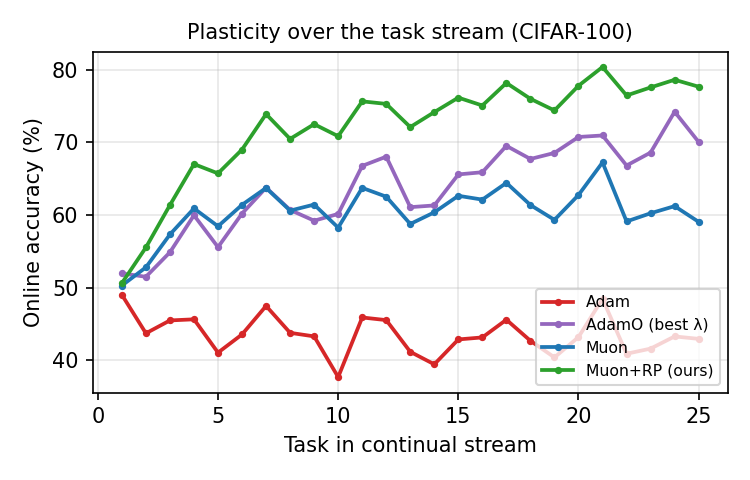
\includegraphics[width=0.92\linewidth]{fig_curves.png}
\caption{\textbf{Plasticity over the task stream} (CIFAR-100). Online accuracy per task. Adam (red) degrades over the stream (loss of plasticity); Muon-based methods (blue, green) \emph{improve} and sustain high accuracy, staying well above AdamO at its best $\lambda$ (purple) throughout.}
\label{fig:curves}
\end{figure}
\begin{figure}[h]\centering
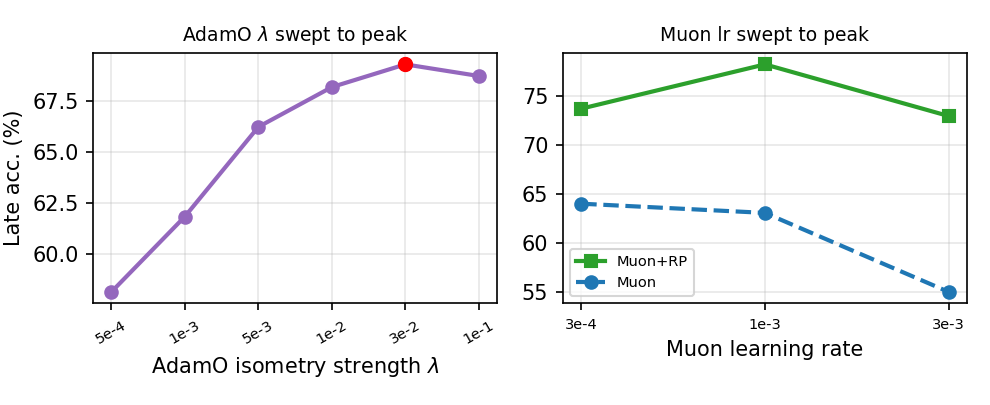
\includegraphics[width=\linewidth]{fig_sensitivity.png}
\caption{\textbf{Both methods are tuned to their peak} (CIFAR-100). Left: AdamO's late accuracy vs.\ isometry strength $\lambda$, peaking at $\lambda{=}3{\times}10^{-2}$; using the default $\lambda$ understates it by up to $11$ points. Right: Muon and Muon$+$RP vs.\ learning rate, peaking at $10^{-3}$. Each method is reported at its own optimum, so the $+9.3$ gap is not a tuning artifact.}
\label{fig:sens}
\end{figure}

\end{document}
